\documentclass[prx,superscriptaddress,twocolumn,nopreprintnumbers,floatfix,nofootinbib]{revtex4}
\usepackage{graphicx,url,amssymb,amsmath,rotating,color,units,wasysym,epsfig,multirow,epstopdf}
\usepackage[colorlinks,urlcolor=blue,citecolor=blue,linkcolor=blue]{hyperref}
\usepackage{soul,xcolor,aas_macros}

\newcommand{\red}[1]{\textcolor{red}{#1}}
\newcommand{\ga}[1]{\textcolor{orange}{[GA: #1]}}
\newcommand{\et}[1]{\textcolor{red}{[ET: #1]}}
\newcommand{\pdl}[1]{\textcolor{red}{[PDL: #1]}}
\newcommand{\bs}[1]{\textcolor{cyan}{[BS: #1]}}
\newcommand{\jvh}[1]{\textcolor{blue}{[JvH: #1]}}
\newcommand{\jl}[1]{\textcolor{red}{[JL: #1]}}
\newcommand{\djo}[1]{\textcolor{purple}{[DO: #1]}}
\newcommand{\vba}[1]{\textcolor{green}{[VBA: #1]}}
%\definecolor{antiquefuchsia}{rgb}{0.57, 0.36, 0.51}
%\newcommand{\swsn}[1]{\textcolor{antiquefuchsia}{[SN:#1]}}
\newcommand{\swsn}[1]{\textcolor{cyan}{[SN:#1]}}
\newcommand{\je}[1]{\textcolor{brown}{[JE:#1]}}

\newcommand{\ozhf}{{\sc OzHF}}


\begin{document}

\title{An extreme matter observatory:\\A high-frequency gravitational-wave interferometer in the global network}

\author{Alphabetical OzGrav author list (opt-out policy)}
\email{coo@ozgrav.org}
\affiliation{}
\affiliation{}

\date{\today}

\begin{abstract}
Gravitational waves from coalescing neutron stars encode information about nuclear matter at extreme densities, inaccessible by laboratory experiments. The late inspiral is influenced by the presence of tides, which depend on the neutron star equation of state.
Neutron star mergers are expected to produce remnant hyper-massive (and/or supra-massive) neutron stars. These rapidly rotating remnants emit gravitational waves, providing clues to the extremely hot post-merger environment—--a likely source for $r$-process (neutron-capture) elements.
The signature of nuclear matter in gravitational waves contains most information in the $\unit[2-4]{kHz}$ frequency band. This is outside of the most sensitive band of current detectors.
We present the design concept and science case for an extreme matter observatory, a gravitational-wave observatory optimized to study nuclear physics with merging neutron stars.
The concept uses high circulating laser power, quantum squeezing and a detector topology specifically designed to achieve the high frequency sensitivity necessary to probe nuclear matter using gravitational waves. 
\end{abstract}

\maketitle

\section{Introduction}
Gravitational-wave astronomy is reshaping our understanding of the Universe.
Recent breakthroughs include the detection of many gravitational-wave signals from binary black hole collisions~\cite{abbott18_O2catalog} leading to an enhanced understanding of their population properties~\cite{abbott18_O2population}, measurement of the Hubble parameter~\cite{abbott17_gw170817_Hubble}, unprecedented constraints on the speed of gravity change~\cite{abbott17_gw170817_gwgrb} and hence the mass of the graviton~\cite{abbott17_gw170104,abbott19_gw170817_grtest}, to name a few.
Plans for building the next generation of observatories are afoot.  The United States National Science Foundation (NSF), Australian Research Council (ARC), and British government have financed A+, an upgrade to Advanced LIGO (aLIGO), which will increase the sensitivity of the current detectors by a factor of 2-3 dependent on the specific frequency of interest.
Research and development is ongoing for third-generation observatories, the Einstein Telescope \cite{punturo2010einstein} and Cosmic Explorer \cite{reitze2019cosmic}; broadband instruments with capabilities of hearing black hole mergers out to the dawn of the Universe.

Third-generation observatories require substantial, global financial investments and significant technological development over many years.
To bridge the gap between A+ and full-scale, third-generation instruments, it is prudent to explore smaller scale facilities that produce significant astrophysical and fundamental physics outcomes, while simultaneously driving technology development.
In this spirit, we introduce an Extreme Matter Observatory (EMO): a dedicated high-frequency gravitational-wave observatory designed to measure the fundamental properties of nuclear matter at extreme densities with gravitational waves.
We envision EMO as a specialized, high-frequency observatory in a heterogeneous network with two or more A+ sensitivity observatories.
The A+ observatories provide source localization while an EMO measures the imprint of extreme matter in gravitational-wave signals from binary neutron star mergers.

%The basic premise of an EMO is to build a detector optimized to high-frequency gravitational waves, where effects of matter during neutron-star mergers dominate. 
Neutron stars are an end state of stellar evolution.
They are the densest known objects in the Universe, and are believed to consist of a superfluid, superconducting core of matter at supranuclear densities.
Such conditions are impossible to produce in the laboratory, and theoretical modelling of the matter requires extrapolation by many orders of magnitude beyond the point where nuclear physics is well understood.
As two neutron stars coalesce, their composition leaves an imprint on the gravitational waveform, which becomes increasingly important at high frequencies $\sim\unit[0.5-4]{kHz}$.

Mergers produce remnants, some of which collapse to black holes, and some of which survive as long-lived, massive neutron stars.
The nature of the remnant is strongly dependent on details of nuclear physics, which is encoded in the neutron star equation of state~\cite[e.g., see][and references therein]{bernuzzi19}.  
Measuring gravitational waves at these high frequencies therefore offers a window into the composition of neutron stars, not accessible with other astronomical observations or terrestrial experiments.  

The technologies that will enable an EMO are key components for third-generation observatories such as Cosmic Explorer. 
In order to reduce quantum shot noise, future detectors aim to employ aggressive squeezing (e.g., up to $\sim\unit[10]{dB}$).  
To enable increased circulating power, reduce scattering losses and reduce thermal noise, future detectors may include cryogenic silicon test masses with high power $\unit[2]{\mu} m$ lasers.
An EMO observatory provides technological development for Cosmic Explorer-like detectors while producing impactful science results on a shorter timescale.

This paper is set out as follows: in Sec.~\ref{sec:design} we lay out the basic design principals of an EMO, including a detector schematic and example noise budget.  Section~\ref{sec:science} details the science deliverables for an EMO; the determination of the neutron star equation of state, and measurement of post-merger remnants.  In Sec.~\ref{sec:conclusion}, we provide concluding remarks and sketch a path forward to a high-frequency detector within the international gravitational wave network.

\section{Design concept}\label{sec:design}
% \begin{itemize}
%     \item Basic principal: high laser power, maximal squeezing, ignore seismic isolation.
%     \item Show design sensitivity curve, then break down technologically specifics. 
%     \item Detector topology; i.e., sketch of detector layout.
%     \item Details of design, includes table of key parameters (e.g., length of SRC, squeezing, \ldots)
%     \item Subsection on risk analysis.  i.e., what may not be achievable.
% \end{itemize}

Simultaneously achieving high sensitivity at low ($\lesssim\unit[50]{Hz}$) and high ($\gtrsim\unit[1]{kHz}$) frequencies in a single detector is extremely challenging. There are two main reasons for this. Firstly, the optical bandwidth of high sensitivity kilometer scale detectors is limited. Thus to achieve sensitivity peaked at 2 kHz requires a loss of optical sensitivity below 500 Hz. Secondly, the high circulating power required to improve high frequency sensitivity introduces opto-mechanical instabilities whose control strategies can easily increase the noise in the low frequency band. Detectors like the Einstein Telescope~\cite{ET} plan to limit low and mid-band frequency noise sources such as thermal noise by operating at $20~\mathrm{K}$ which is not compatible with high circulating power.
Proposals for the third-generation Einstein Telescope~\cite{ET} circumvent this by building multiple detectors in a common subterranean vacuum envelope. In our EMO we plan to only concentrate on the frequency regime above $1~\mathrm{kHz}$, sacrificing low-frequency sensitivity and thereby decreasing engineering challenges and cost. We assume that the low frequency sensitivity required for sky localization will be achieved by the other detectors in the network.

Martynov et al.\cite{martynov19} have shown that the optimal length of a high frequency detector is 16~km. At this time it is unlikely that the funds needed to build a dedicated high frequency detector of this scale could be obtained, hence we have compromised to an arm length of 4 km. This arm length is sufficient to prevent displacement noise sources causing concern without being prohibitively expensive to build. This reduction in arm length reduces the maximum sensitivity that can be obtained by a factor of 2 which may in principal be recovered in a future upgrade using a folded interferometer as outlined in \cite{ballmer2013new}. 

Our approach for achieving high frequency sensitivity in the EMO comparable to third generation gravitational wave observatories is outlined below. A simplified schematic of the inteferometer is illustrated in Fig. \ref{detector_design} and the design parameters are included in Table ~\ref{tab:design}.

The high frequency sensitivity of an interferometric gravitational wave detectors is predominantly limited by quantum phase noise which is due to the quantum nature of light and not displacement noise sources such as seismic and thermal. Increasing the circulating power within the detector reduces this quantum phase noise proportional to the inverse of the square root of the power \cite{martynov19}.  Therefore to maximize the sensitivity the circulating power in the arms must be as high as possible. This quantum phase noise source can also be reduced by injecting squeezed vacuum into the dark port \cite{aasi2013enhanced}. As a baseline design we have chosen to use $4.6~\mathrm{MW}$ circulating power in the arms and $10~\mathrm{dB}$ of squeezing to further enhance sensitivity. 

The quantum phase noise limited nature of high frequency interferometers means that there are unlikely to be significant advantages in using exotic interferometer types such as speed meters or other Sagnac style interferometers. For this reason we have chosen a dual recycled Michelson interferometer design with Fabry-Perot arm cavities, similar to current interferometric gravitational wave detectors~\cite{aasi2015advanced,acernese2014advanced,aso2013interferometer}. However there are some key differences targeted to maximise the sensitivity in the 1~kHz to 5~kHz signal band of interest, while maintaining relatively short arm cavities.

The signal recycling cavity and the arm cavity of the interferometer form a coupled cavity system which determines the overall bandwidth of the interferometer. For the EMO, the transmission of the input test mass was set to 1.4\% to obtain 4.6~MW in the arm cavity. In order to maximise the sensitivity of the EMO in the 1~kHz to 5~kHz frequency band of interest, the length of the signal recycling cavity was optimised using numerical simulation tools namely PyKat and Finesse~\cite{Finesse,finesse1,brown2020pykat} to be 354\,m. This 'long' signal recycling cavity displays the characteristic splitting of a coupled cavity system~\cite{DEM95,martynov19} around the interferometer carrier frequency where the gravitational wave signal sidebands are resonantly enhanced. This splitting frequency is given by,
	\begin{equation}
	\mathrm{f_{sp}} = \frac{\mathrm{c} \sqrt{\mathrm{{T_{ITM}}}}}{4 \pi \sqrt{\mathrm{L_{arm}}\mathrm{L_{src}}}},
	\label{eqn1}
	\end{equation} 
	where $\mathrm{T_{ITM}}$ is the power transmissivity of the input test mass, and $\mathrm{L_{arm}}$ and $\mathrm{L_{src}}$ are the lengths of the arm cavities and the signal recycling cavity respectively. The bandwidth $\gamma$ of this coupled cavity system depends on the transmission of the signal recycling mirror (SRM) as well as the length of the SRC.
 
 The same effect of enhanced sensitivity at certain frequencies can be obtained by detuning the signal recycling cavity~\cite{SRCdetuned}. This configuration however comes with technical challenges pertaining to the control of the interferometer.

Cryogenically-cooled silicon test masses will be used to maximise the potential circulating arm powers prior to adverse thermal distortions. At cryogenic temperatures silicon exhibits high thermal conductivity and low thermal expansion~\cite{kim2018} while also providing reduced thermal coating noise~\cite{shapiro2017cryogenically}. These test masses necessitate a departure from the $\unit[1.06]{\mu m}$ lasers used in the current generation of gravitational wave detectors. 
An EMO operating with a $500~{W}$ $\unit[2]{\mu m}$ single frequency diffraction limited laser has been specified based on the silicon transmission window, the potential for reduced test-mass coating absorption~\cite{steinlechner2018}, and the relative technological maturity of prospective sources.
Thulium-doped fibre lasers have been selected as the laser candidate due to their intrinsic beam quality, demonstrated narrow linewidths at high power~\cite{goodno2009} and potential for robust all-fibre architecture. While fibre laser technology has been demonstrated at $200~W$ at $\unit[1]{\mu m}$ with the required intensity and frequency noise~\cite{ buikema2019, wellmann2019} this has not yet been demonstrated at $\unit[2]{\mu m}$. Fortunately, the thresholds of non-linear processes that limit the maximum power level of single frequency fibre lasers increase faster than the wavelength squared~\cite{dawson2008}, hence it seems likely that $500~W$ of power required for an EMO will be demonstrated in the near future.

In order to obtain the sensitivity target of the EMO without further increasing the arm cavity power, introducing squeezed light is essential. For this purpose, we will inject 10~dB of frequency independent squeezing into the interferometer. In the frequency range of 1~kHz to 5~kHz only quantum phase noise suppression is required so systems to rotate the suppression quadrature to quantum radiation pressure noise reduction such as filter cavities are not required. The 10~dB injected squeezing assumed here is realistic as a 6~dB reduction in quantum shot noise in a kilometer scale detector (GEO\,600~\cite{squeezeRecord_GEO2018}) has already been demonstrated. 

\begin{figure}[htb]
\centering
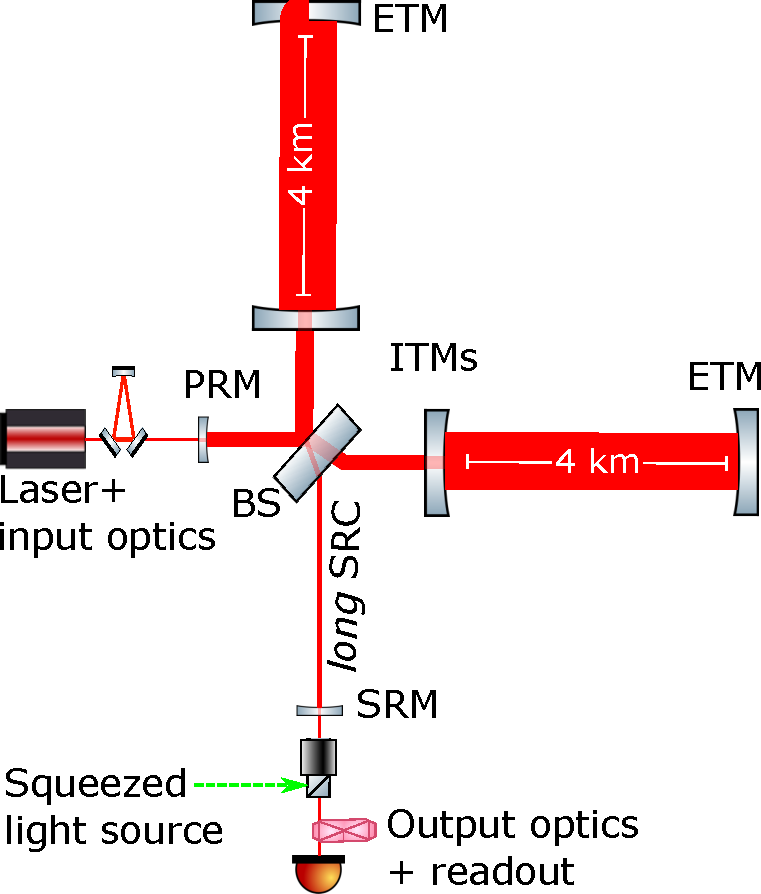
\includegraphics[width=0.5\textwidth]{GenGWDoverviewLongSRC}
\caption{Simplified optical topology of EMO. Folding of the recycling cavities, input and output optics, e.g. various mode cleaners, not shown for clarity. A summary of the design parameters is included in Table \ref{tab:design}
}
\label{detector_design}
\end{figure}


\begin{table}[]
    \centering
    \begin{tabular}{c c}
    
         Parameter & Value \\
         \hline
        \hline
         Laser Wavelength & $ 2~\rm{\mu m}$ \\
         Laser Power & 500 W \\
         Arm Length & 4 km \\ 
         Losses & 20~ppm/cm (ea) \\
         PRM Transmission & 3\% \\
         ITM Transmission & 1.4\% \\
         ETM Transmission & 5~ppm \\
         SRM Transmission & 4.8\% \\
         Bean spot radius on ITM & 57.9~mm\\
         Bean spot radius on ETM & 83.9~mm\\
         Power on Beamsplitter & 32~kW \\
         Arm Circulating Power & 4.6~MW \\
         Injected Squeezing level & 10~dB \\
         Test mass material & Silicon \\
         Operating Temperature & 123 K \\
         Signal recycling cavity length & 354~m \\
         Test mass coating & AlGaAs/GaAs \\
         Test mass weight & 94.4~kg \\
         Test mass diameter & 45~cm \\
         Suspension fibre length &	0.55~m \\
         Suspension fibre material & steel \\
         Suspension fibres per test mass &	4 \\
         TM cooling method & Radiative \\
         Interferometer Configuration & Dual Recycled with FP arms \\
         \hline
    \end{tabular}
    \caption{All recycling cavities are stable cavities.
    }
    \label{tab:design}
\end{table}

The focus on high frequency performance means that requirements on the suspension and seismic isolation systems are not onerous. The in-band noise performance could likely be achieved using the seismic isolation and the steel suspension system used in the initial LIGO interferometer \cite{abbott2009ligo}. Further, to reduce the peak velocity of the optics in the pre-locked state all the main optics are suspended by a multi-stage suspension and isolation systems. For the science objectives presented below we have assumed that no sensitivity is achieved below 500 Hz.

The performance of the second generation detectors will be limited by coating thermal noise in the mid-band around 100 Hz once design sensitivity has been reached. The order of magnitude improvement in quantum noise promised by HF detectors promotes the coating thermal noise levels seen in current detectors to become a limitation at kHz frequencies, where it used to be of little concern. The constraints on coatings are further increased due to the requirement that coating absorption is very low.

Two potential coating choices are being actively researched for use in cryogenic third generation detectors. The two promising coatings are epitaxially grown single-crystal coatings and ion-beam sputtered amorphous mirror coatings. The crystalline coatings use either AlGaAs/GaAs~\cite{cole2008algaas,cole2013algaas-nature,penn2019algaas} or AlGaP/GaP~\cite{lin2013algap,cumming2015algap,murray2017algap} as alternating multi-layer. The amorphous coatings are alternating layers of Silicon and Silicon Oxide in a multi-layer configuration~\cite{steinlechner2016aSi,birney2018aSi}.

Currently, the choice of coatings is not clear cut as the amorphous coatings have a thermal noise advantage but suffer from unacceptably high loss (20 ppm). The AlGaAs/GaAs coatings suffer from elevated levels of thermorefractive noise principally due to the high thermorefractive coefficient of GaAs. With careful coating design this noise source can cancel with thermoelastic noise. 

Our modelling (see Fig.~\ref{fig:noisecurve}) assumes an AlGaAs/GaAs multi-layer coating as per current best measured characteristics or mentioned otherwise whenever e.g. interpolated in the following discussion. 

We have chosen to operate the interferometer at 150 K rather than the 123 K specified for other third generation silicon designs. This is to allow the high power that will be absorbed to be radiatively dissipated to the 77 K cooled shields that will surround the test masses and not have to resort to conductive cooling \cite{Eichholz2020} that is complicated and can compromise the suspension thermal noise of the detector. The details of this design are outlined in a companion paper \cite{Eichholz2020} and are summarized below.

The stored optical power in the arm cavities will be $4.5~MW$, comparable to the Cosmic Explorer and Voyager designs of $3~MW$ \cite{reitze2019cosmic}\cite{voyager-arxiv}. The transition to silicon test masses will benefit performance in the same way as other third-generation instruments. The higher thermal conductivity, along with the prospect of operating with low substrate thermal expansion offers an attractive solution to the high-power problem. At the same time, a silicon-based cryogenic detector would profit from the same advancements in coating technology that are being pushed for the development of third-generation gravitational-wave detectors. 

Silicon at a temperature in the range of $120-150~K$ has a low thermal expansion coefficient and a very high thermal conductivity meaning that thermal distortion of the mirror surfaces is reduced to very low levels. The thermooptic coefficient of silicon is higher than that of room temperature silica that is used in the current detectors. However, the dramatically increased thermal conductivity of silicon means that the thermal lensing in the substrates will be considerably reduced despite the greater absorption in silicon substrates compared with a comparable room temperature silica detector. Point absorbers on the high reflectivity surfaces of the test masses have caused significant local distortions of these surfaces in the aLIGO detector \cite{LIGO_O3_DET}. The impact of point absorbers will be reduced by a factor of over 300 for a silicon interferometer operating at 150 K compared with a silica interferometer operating at room temperature \cite{Eichholz2020}.

To maximise the surface area for radiative heat transfer we assume a mirror diameter of 45 cm, which is projected to become available in the form of single crystal cylindrical silicon boules grown by a magnetically-assisted Czochralski method (m-Cz) for semiconductor applications~\cite{lin2008_silicon}. Absorption levels of 10 ppm/cm have been demonstrated in m-Cz silicon~\cite{voyager-arxiv}. A thickness of 26.5 cm approximates the Advanced LIGO aspect ratio of 1.7, and results in a total mass of 98.2 kg. A black body of equivalent dimensions, held at 123 K, thermally radiates a total power of 9 W into its environment. At 150\,K, this increases to 20\,W. We assume that a cooling rate of about 70\% of these values can be achieved, as shown by detailed finite element simulations for Voyager~\cite{voyager-arxiv}, resulting in 6.3\,W and 13.9\,W, respectively.

A heat load of 5 W on the test masses is expected from a residual 1 ppm absorption of the HR coatings with 5 MW of circulating power in the arms. Heating due to the transmitted light in the ETMs is negligible, however, with 31 kW incident on the beamsplitter, and each beam performing a double-pass through its respective ITM, the bulk heating power becomes 0.31 W/cm, for a total of 8.2~W. An elevated temperature of 150 K for the input test masses is therefore selected. More details on this elevated temperature operation can be found in \cite{Eichholz2020}. Summarising, we can state that radiatively cooling the input test mass, considering the heat load by absorption, needed an elevated temperature to increase the thermal gradient between test mass and cold shield. A trade-off between this and increased thermal lensing and low-frequency thermal noise were modelled to finally result in an optimum temperature of 150 K. 

The beam splitter material choice is still an open question. The 31 kW that is incident on the beam splitter will result in significant astigmatic thermal lensing even when the absorption in the substrate is low. In this situation, as with the GEO600 detector \cite{Wittel18_BSComp} the beam splitter will need to be compensated. Different schemes to provide this compensation are actively being investigated.  

Experience with current gravitational wave detectors has shown that  opto-mechanical instabilities arise when operating with high circulating powers, such as parametric instabilities \cite{evans2015observation}, and angular misalignment \cite{sidles2006optical},\cite{hirose2010angular}. The high circulating power inside the arm cavities could make the EMO quite sensitive to opto-mechanical instabilities. However, this is where the dedicated high frequency nature of the detector really comes into it own. 

In the case of angular instabilities, the bandwidth of the angular control loops can be significantly increased beyond what can be used for broadband detectors.  Modeling has shown even at $5~MW$ of circulating power the coupled opto-mechanical tilt modes of the EMO arm cavities will not exceed 15 Hz. Recently developed techniques will be implemented to mitigate these effects \cite{amd}. These show that tilt modes can be controlled with angular control bandwidth of $\sim$3x the modified mode frequency, with sufficient noise suppression ($>60~\text{dB}$) at $\sim$10x the modified mode frequency\cite{LIGO-T1400226} \cite{barsotti_2010}. Hence the noise injected by the required angular control loops should be insignificant for frequencies beyond 1kHz. \djo{Fix references}
 

Parametric instability was first observed at aLIGO with about 40~kW \cite{Evans2015_PI} circulating power in the arms while aVIRGO did not observed parametric instabilities with circulating power of around 100~kW in 2019. This is indicative of the high sensitivity of parametric instability to cavity and test mass parameters, detailed models are required for accurate prediction of parametric instability.  This detailed analysis is currently being performed \cite{Juntao2020}.  However rough estimation can be performed by assuming a scaling of aLIGO parameters and related scaling of the severity of parametric instabilities described in \cite{Braginsky01}.
Parametric instability severity scales proportional to circulating power and optical quality factors and inversely proportional to mirror mass and mechanical eigenfrequencies.  The power will be 125 times higher than where aLIGO first observed parametric instability, the optical quality factors will be 1.35 times higher, the mirror mass will be 2.5 times heavier, and the lowest mechanical frequency is 1.2 times higher.  If other parameters are considered unchanged, parametric instability is expected to be 56 times worse than aLIGO with 40~kW circulating power from this scaling argument.  However thermal tuning \cite{Zhao_2006_Therm,Hardwick2020_DTC} allowed optical power to be increased by a factor of 4.3 at aLIGO.  Resonant mass dampers attached to the test masses have been demonstrated to reduce mechanical mode quality factors by 10-100 \cite{Biscans2019_AMD}, introducing negligible thermal noise and electrostatic actuation has been demonstrated to to reduce parametric gain by a factor of 13 and is inferred to be strong enough to reduce mode quality factors by 1000’s \cite{Blair_2017_ESDPI} at 40~kW.  This leads us to believe that with proper consideration of parametric instability and its mitigation it may be controlled in EMO.



\begin{figure}[htb]
\centering
% 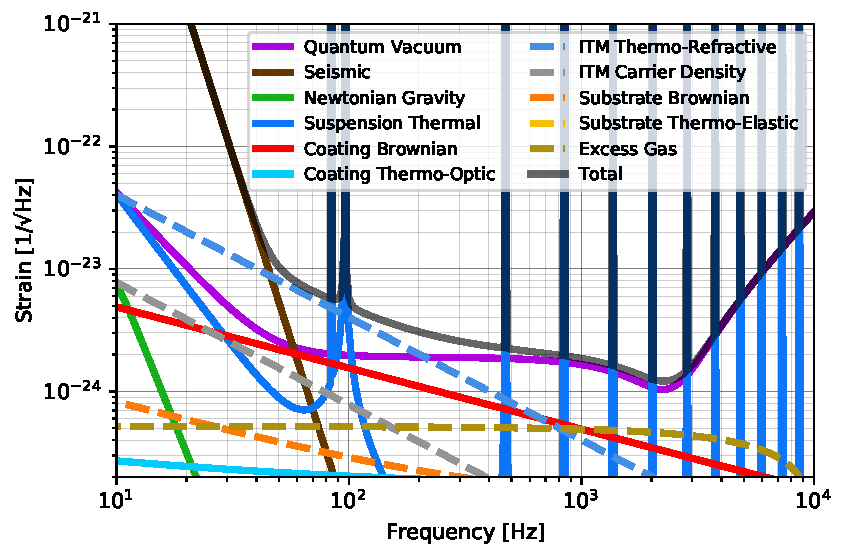
\includegraphics[width=0.5\textwidth]{OzHF_noisebudget2.pdf}
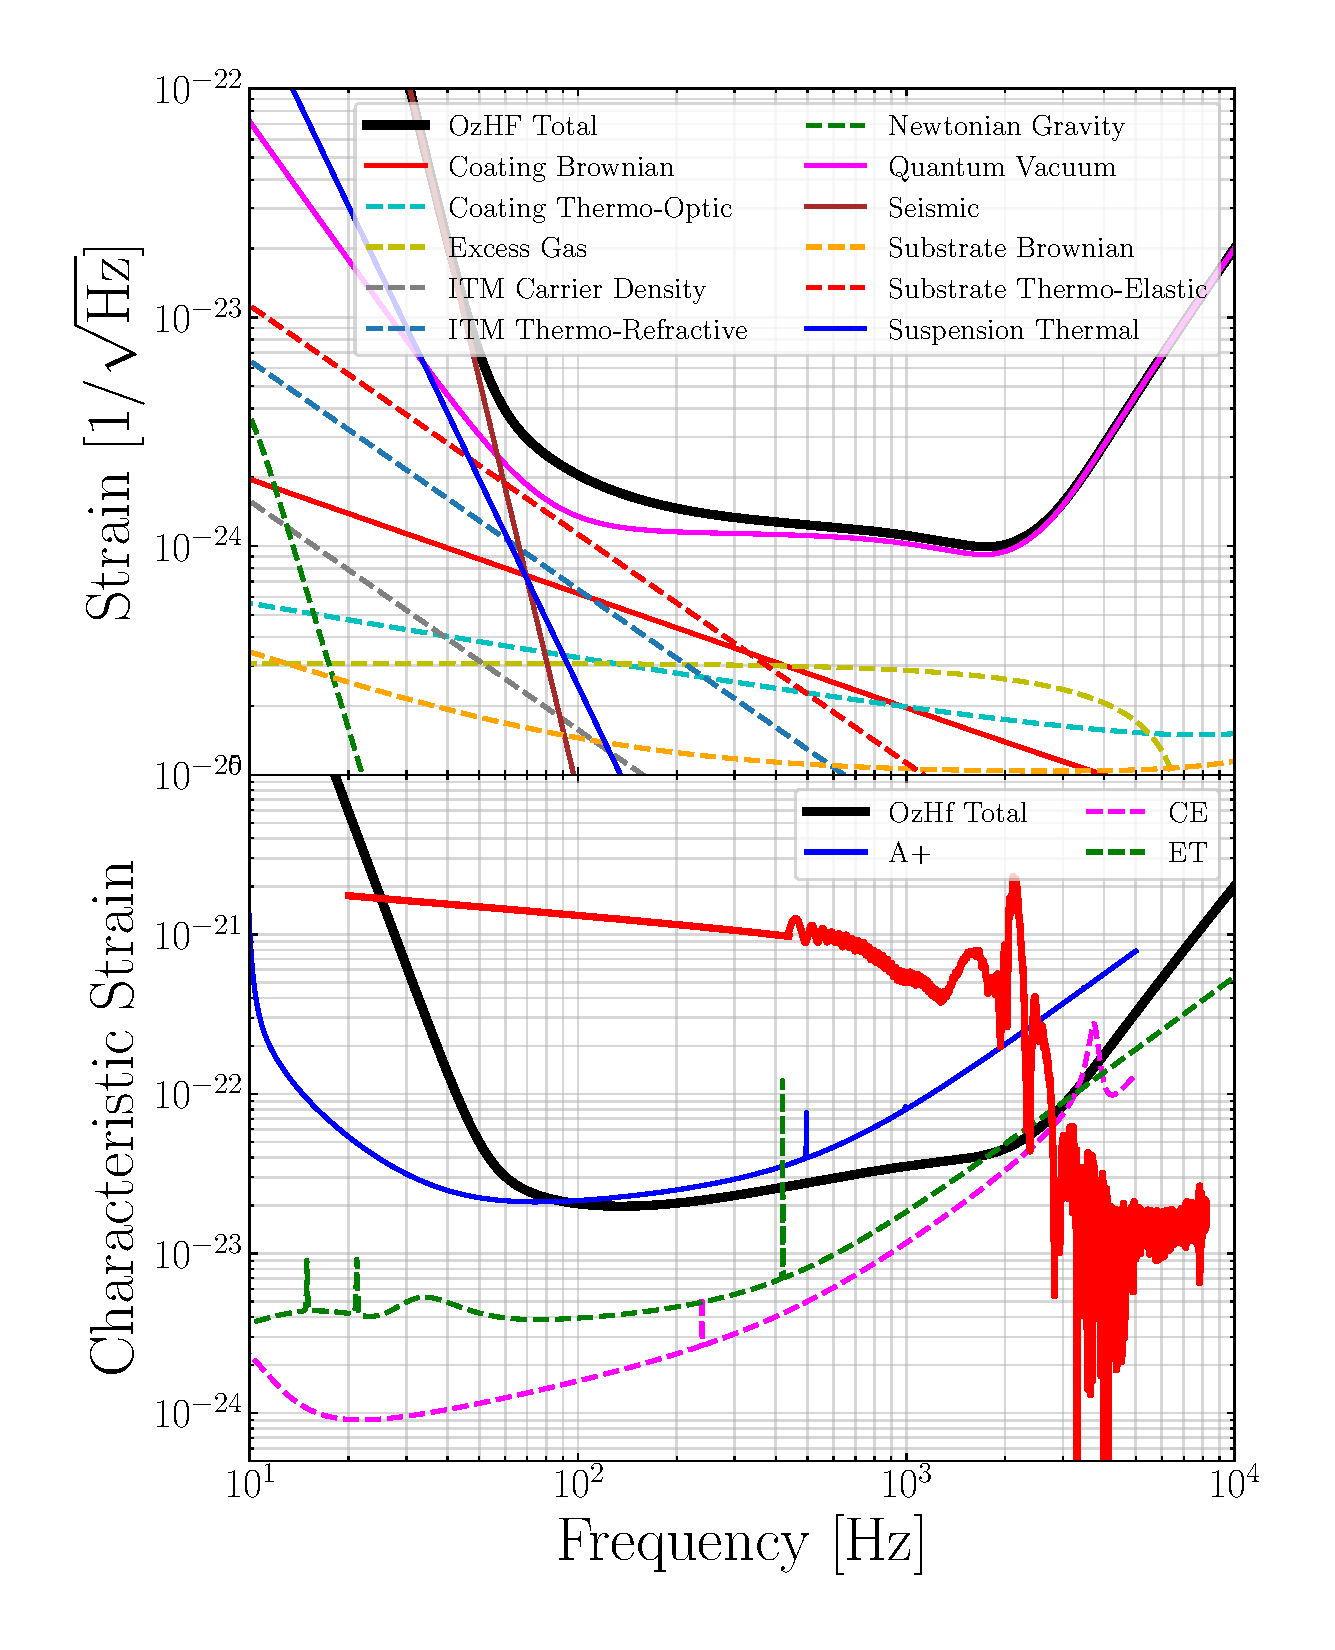
\includegraphics[width=1.0\columnwidth]{noise_budget_hc.pdf}
\caption{Noise budget and indicative gravitational-wave signal from a binary neutron star collision.  Top panel: we show the amplitude spectral density of the various noise components that make up the total noise budget shown as the black curve.  Bottom panel: The black curve is the same total noise budget as the top panel, now shown as the noise amplitude $h_n=\sqrt{fS_n(f)}$, where $S_n(f)$ is the power-spectral density. This curve is shown in comparison to design sensitivity of A+ (blue), the Einstein Telescope (ET; green), and Cosmic Explorer (CE; pink).  Also shown in red is the characteristic gravitational-wave strain $h_c$ for a typical binary neutron star inspiral, merger, and post-merger at 40 Mpc.}
\label{fig:noisecurve}
\end{figure}


\section{Scientific deliverables}\label{sec:science}

To motivate the science case for an EMO, we discuss physics encoded in the high-frequency gravitational-wave emission during both the inspiral and post-merger phases of a binary neutron star merger.
These two phases probe different temperature regimes of the neutron star equation of state.
During inspiral, neutron stars are relatively cold, with temperature $T\ll\unit[10^{9}]{K}$, having had sufficient time to cool since birth.  
Under such conditions, the temperature does not significantly affect internal physical structure that determines bulk stellar quantities such as the stellar radius.  
Temperatures during merger can reach as high as $T\sim\unit[10^{11}]{K}$~\cite[e.g.,][]{Baiotti2008,foucart16}, and can therefore affect the equation of state. 


\subsection{The physics of cold neutron stars}
For cold neutron stars in the pre-merger phase, the tidal deformation of the individual components is imprinted in the gravitational-wave emission.  The tidal deformation is dependent on the EOS, and is parameterized by the ``combined dimensionless tidal deformability'' $\tilde\Lambda$, given by:
\begin{align}
    \tilde\Lambda \equiv \frac{16}{13}\frac{(m_1+12m_2)m_1^4\Lambda_1+(m_2+12m_1)m_2^4\Lambda_2}{(m_1+m_2)^5}.
\end{align}
Here $m_1$ and $m_2$ are the masses of the component neutron stars, and $\Lambda_1$ and $\Lambda_2$ are the tidal deformabilities of each neutron star, defined as
\begin{align}
    \Lambda_i\equiv\frac{2k_{2,i}}{3}\left(\frac{c^2R_i}{GM_i}\right)^5,
\end{align}
where $M$, $R$, and $k_{2}$ are the mass, radius, and second Love number.
Gravitational-wave astronomers measure $\tilde\Lambda$ because it is the leading-order correction to gravitational waveforms due to tides.
For a fixed mass, both $R$ and $k_2$ are determined by the neutron star equation of state.
Large values of $\Lambda$ imply soft equations of state, corresponding to small, compact neutron stars.  Small values of $\Lambda$ imply stiff equations of state, where neutron stars are large and comparatively fluffy.
Black holes have $k_2=0$, implying the tidal deformability also vanishes.

A key goal in nuclear astrophysics is to measure the tidal deformability as a function of neutron star mass.  
These tidal effects become increasingly important when the two neutrons stars are close to one another, which occurs late in coalescence and therefore at high gravitational-wave frequencies.
In the bottom panel of Fig.~\ref{fig:noisecurve}, we plot the EMO (black) and A+ (blue) noise amplitude curves $h_n(f)=\sqrt{fS_n(f)}$, where $S_n(f)$ is the detector power spectral density, alongside the gravitational-wave characteristic strain $h_c=2f\tilde{h}(f)$ from the inspiral and postmerger phase of an equal-mass binary neutron star coalescence at \unit[40]{Mpc} (red).  With these quantities, the signal-to-noise ratio $\rho$ is simply~\cite[e.g.,][]{moore15}
\begin{align}
    \rho^2=\int_{-\infty}^\infty d\ln f\left(\frac{h_c(f)}{h_{n}(f)}\right)^2.
\end{align}
Tidal effects become important at frequencies $\gtrsim\unit[400]{Hz}$~\cite{harry18}; at that point, the gravitational waveforms describing a binary black hole system and a binary neutron star system begin to dephase.  The most sensitive region of an EMO is designed to be sensitive to the physics of this late inspiral phase.


% \begin{figure}[htb]
% \centering
% 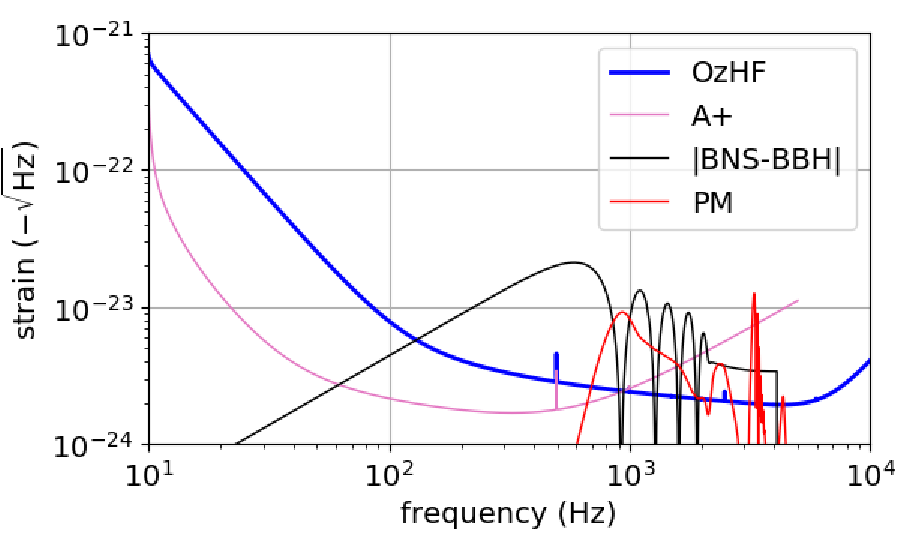
\includegraphics[width=0.5\textwidth]{noisecurve}
% \caption{
% \et{Update this plot to include the most recent an EMO noise curve.} \jvh{Maybe go for same look as our noise budget, at least have a full loglog grid like noise budget. Maybe these figures are 2a and 2b?}
% The sensitivity of OzHF to matter effects in neutron stars.
% Blue is the noise amplitude spectral density of OzHF.
% Purple is the noise amplitude spectral density for A+ (REF).
% Black is the characteristic strain of the tidal signature in the binary neutron star signal (see the text for details).
% Red is the characteristic strain for the post-merger remnant.\et{Eric and Paul: update the plot to use just amplitude spectral density.
% Fix the post-merger waveform so that it is scaled to the appropriate distance.}
% }
% \label{fig:noisecurve}
% \end{figure}

To study the sensitivity with which an EMO can measure tidal deformability, we perform a Monte Carlo study in which we inject binary neutron star inspiral signals into simulated noise from two different detector networks.
Network I consists of two A+ detectors located at Hanford and Livingston, and the Network II is a three-detector network that adds an an EMO observatory.
We assume the following population properties: (1) uniform in co-moving volume; (2) uniform in chirp mass between ${\cal M}_c \in 1.05-1.45 M_\odot$; (3) uniform in mass ratio between $q \in 0.9-1$, (4) aligned spin between XYZ, (5) $\tilde\Lambda$ determined by the SLy equation of state~\cite{douchin01}.

Using the Bayesian inference library Bilby~\cite{ashton19}, we measure the masses and tidal deformabilities, and reconstruct the equation of state following Refs.~\cite{lackey15,hernandez19}.
In Fig.~\ref{fig:mass_radius}, we show a  reconstruction of the mass-radius relation using the loudest five neutron star mergers.
The dashed-blue, grey, and green contour show respectively the 90\% credible interval obtained using the current network of gravitational-wave interferometers operating at design sensitivity, Network I, and Network II (i.e., adding an EMO).  The inclusion of an EMO provides an approximately \red{$50\%$} improvement in the accuracy with which the equation of state can be measured, with the precision comparable to that which can be achieved using complementary X-ray timing observations~\cite[e.g.,][]{bogdanov19}.

\begin{figure}[htb]
\centering
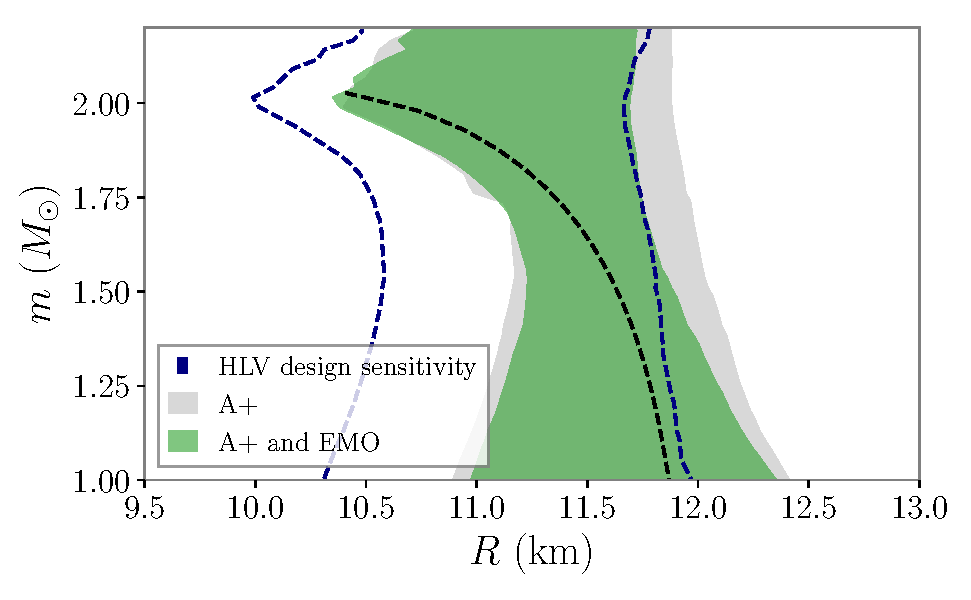
\includegraphics[width=0.5\textwidth]{mass_radius.pdf}
\caption{
Reconstruction of the neutron-star mass radius relation using simulated data from $40$ binary neutron star mergers.
The true relation is shown with the black dashed line.
The blue contour shows the 90\% credible interval obtained with the current network of Advanced LIGO Hanford and Livingston, and Advanced Virgo operating at design sensitivity. The grey contour shows the 90\% credible interval obtained using a network of two A+ interferometers, while the green shows the same interval obtained when an EMO is added to the network.
}
\label{fig:mass_radius}
\end{figure}

\subsection{The physics of hot neutron stars}
Following the merger of two neutron stars, a new compact object is created.  Depending on the remnant mass, this compact object can be a black hole or a massive neutron star.  
In the former case, gravitational-wave emission is difficult to observe because of the relatively short damping time and high frequency $\gtrsim\unit[6]{kHz}$. 
However, if a neutron star survives the merger, gravitational waves can be emitted at frequencies of $\sim\unit[1-4]{kHz}$ for up to hundreds of milliseconds~\cite{Baiotti2008,Shibata2006}.
% Note on refs: tons of refs for PM simulations, don't know how many to cite

The spectral content of the post-merger gravitational waves contains information about the neutron star equation of state~\cite{takami15}.
Following merger the temperature becomes an important equation-of-state parameter.
For example, temperature-dependent phase transitions may occur in the core of post-merger neutron stars.  Measuring gravitational waves from the inspiral and post-merger phase could provide a unique opportunity to identify phase transitions from hadronic matter to deconfined quark matter~\cite{Bauswein2019}.
Furthermore, as the remnant is supported by differential rotation the resulting neutron star in the post-merger phase has a higher density than the component neutron stars from the pre-merger phase.  Thus gravitational-wave emission from the post-merger phase affords the opportunity to prove the EOS in a different density regime.


The precise signal morphology of neutron star post-merger gravitational waves remains unknown. However, numerical simulations have shown that the spectra of the emission from a hyper-massive neutron star remnant contain a characteristic peak frequency, which is approximately equal to the fundamental quadrupolar mode of that neutron star~(REFs).

Using an algorithm that reconstructs gravitational-wave signals as a sum of sine-Gaussian wavelets called \textsc{BayesWave}~\cite{BayesWave}, the post-merger waveform can be reconstructed with minimal assumptions on the exact morphology of the signal.  From this reconstruction, it is possible to produce posterior distributions of the characteristic peak frequency.
For signals with matched filter signal-to-noise ratio $\rho_\text{mf}\gtrsim5$ the peak frequency can be constrained to within tens of Hz~\cite{Chatziioannou,TorresRivas}.

In Fig.~\ref{fig:post-merger}, we show an example of a reconstructed post-merger signal for an event like GW170817 obtained using the \textsc{BayesWave} algorithm following Ref.~\cite{Chatziioannou}.
The top panel shows the 90\% credible interval obtained with Network I (two A+ observatories) and the bottom panel shows the 90\% credible interval obtained with Network II (adding an EMO).
Qualitatively, without an EMO the signal reconstruction losses track of phase of the signal after a few milliseconds, while the reconstruction with an EMO correctly tracks the phase throughout the $\gtrsim\unit{10}[ms]$.  Quantitatively, we see a $\red{X}\%$ improvement in the reconstruction of the peak gravitational-wave frequency.


%The addition of an EMO improves inference of the peak frequency by a factor of \red{XYZ}.

% Notes from Meg:
%   Should we also include example plot of posterior on fpeak/radius?
%   Could also do something similar to Fig. 10 of Torres-Rivas paper
%   (i.e. showing how 90% CI changes vs relative sensitivity. not sure exactly what to put on x-axis though)

\begin{figure}[htb]
\centering
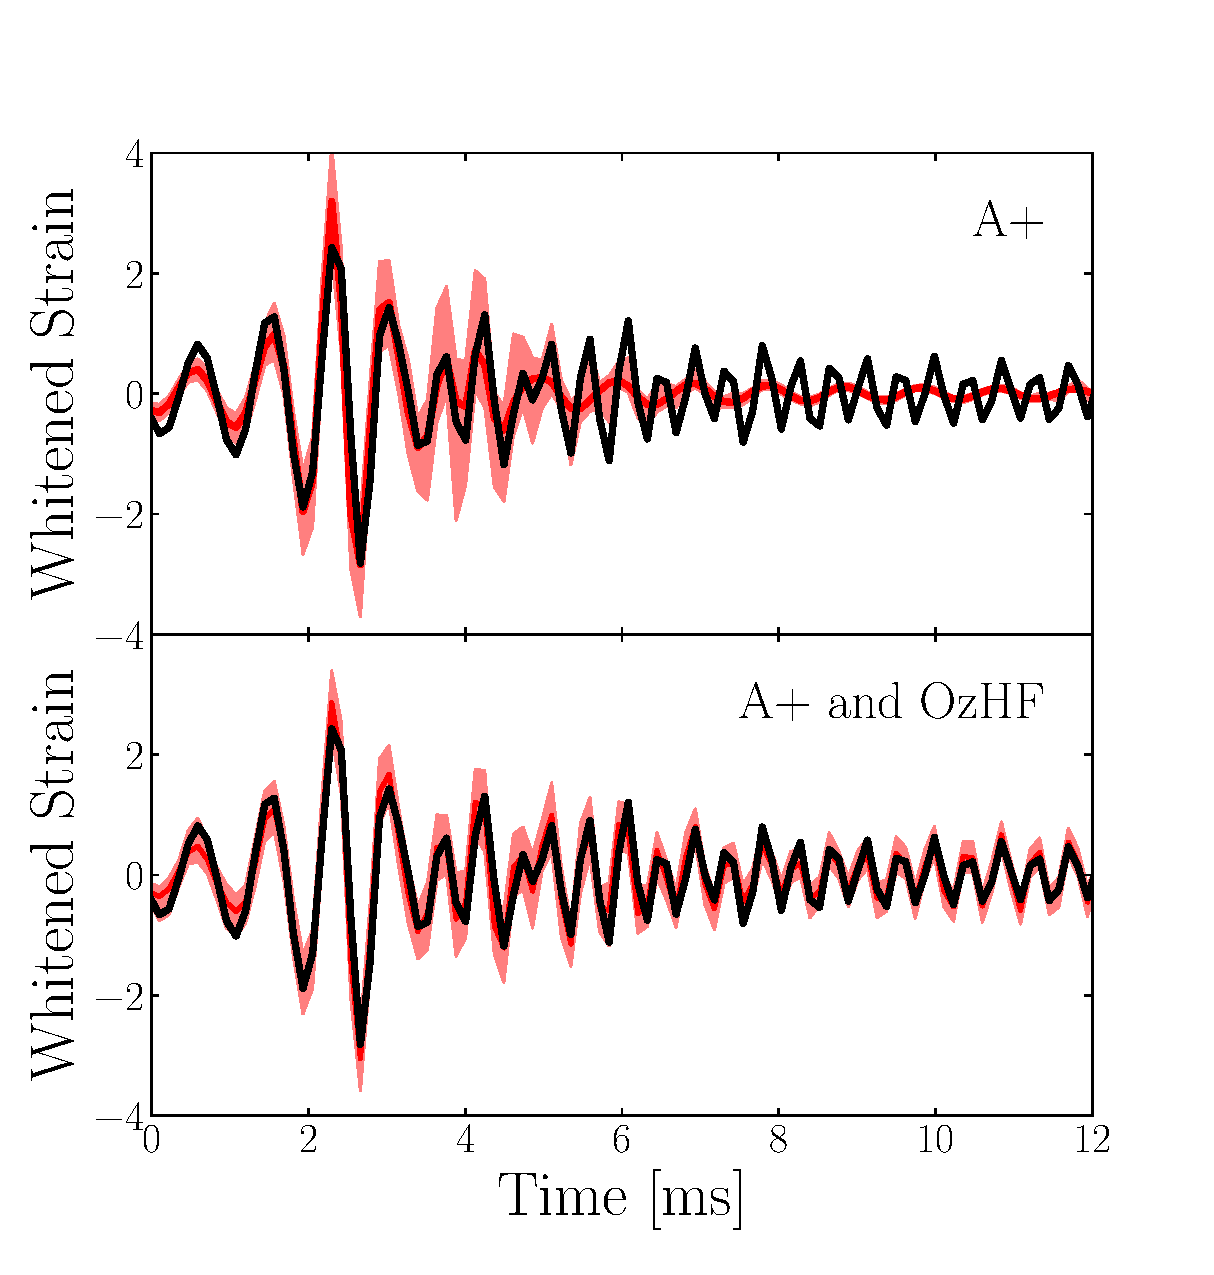
\includegraphics[width=0.5\textwidth]{BayesWaveTimeSeries.pdf}
\caption{Gravitational-wave reconstruction of a post-merger signal with and without an EMO.  We inject the same numerical-relativity post-merger waveform as Fig.~\ref{fig:noisecurve} into a detector network consisting of two A+ detectors (top panel), and two A+ detectors and an EMO detector (bottom panel).  The purple curve shows the injected signal, while the shaded regions show the 90\% confidence interval reconstruction.  Without an EMO, the signal reconstruction fails to track the phase of the signal, whereas the reconstruction with EMO correctly reconstruct the gravitational-wave phase throughout the signal duration.}
\label{fig:post-merger}
\end{figure}

In order to showcase the advantage gained by an EMO, we plot in Fig.~\ref{fig:ndet} the number of expected post-merger events per year for Network I with two A+ observatories (dashed blue) and Network II, which adds an EMO (solid red).
We calculate the matched-filter signal to noise for different signal injections of numerical-relativity post-merger waveforms for a realistic distribution of source distances, orientations, etc, and then calculate the average number of detections (defined as having $\rho_{\rm mf}>5$) per year in either network.
The results are plotted as a function of peak frequency, which depends on the equation of state.
%From lower to higher frequency, we use the following equations of state: MS1b~\cite{MS1b} and SLy~\cite{SLy}.
The length of each line indicates the 90\% credible interval due to uncertainty in the binary neutron star merger rate~\cite{GW190425}.

\begin{figure}[htb]
\centering
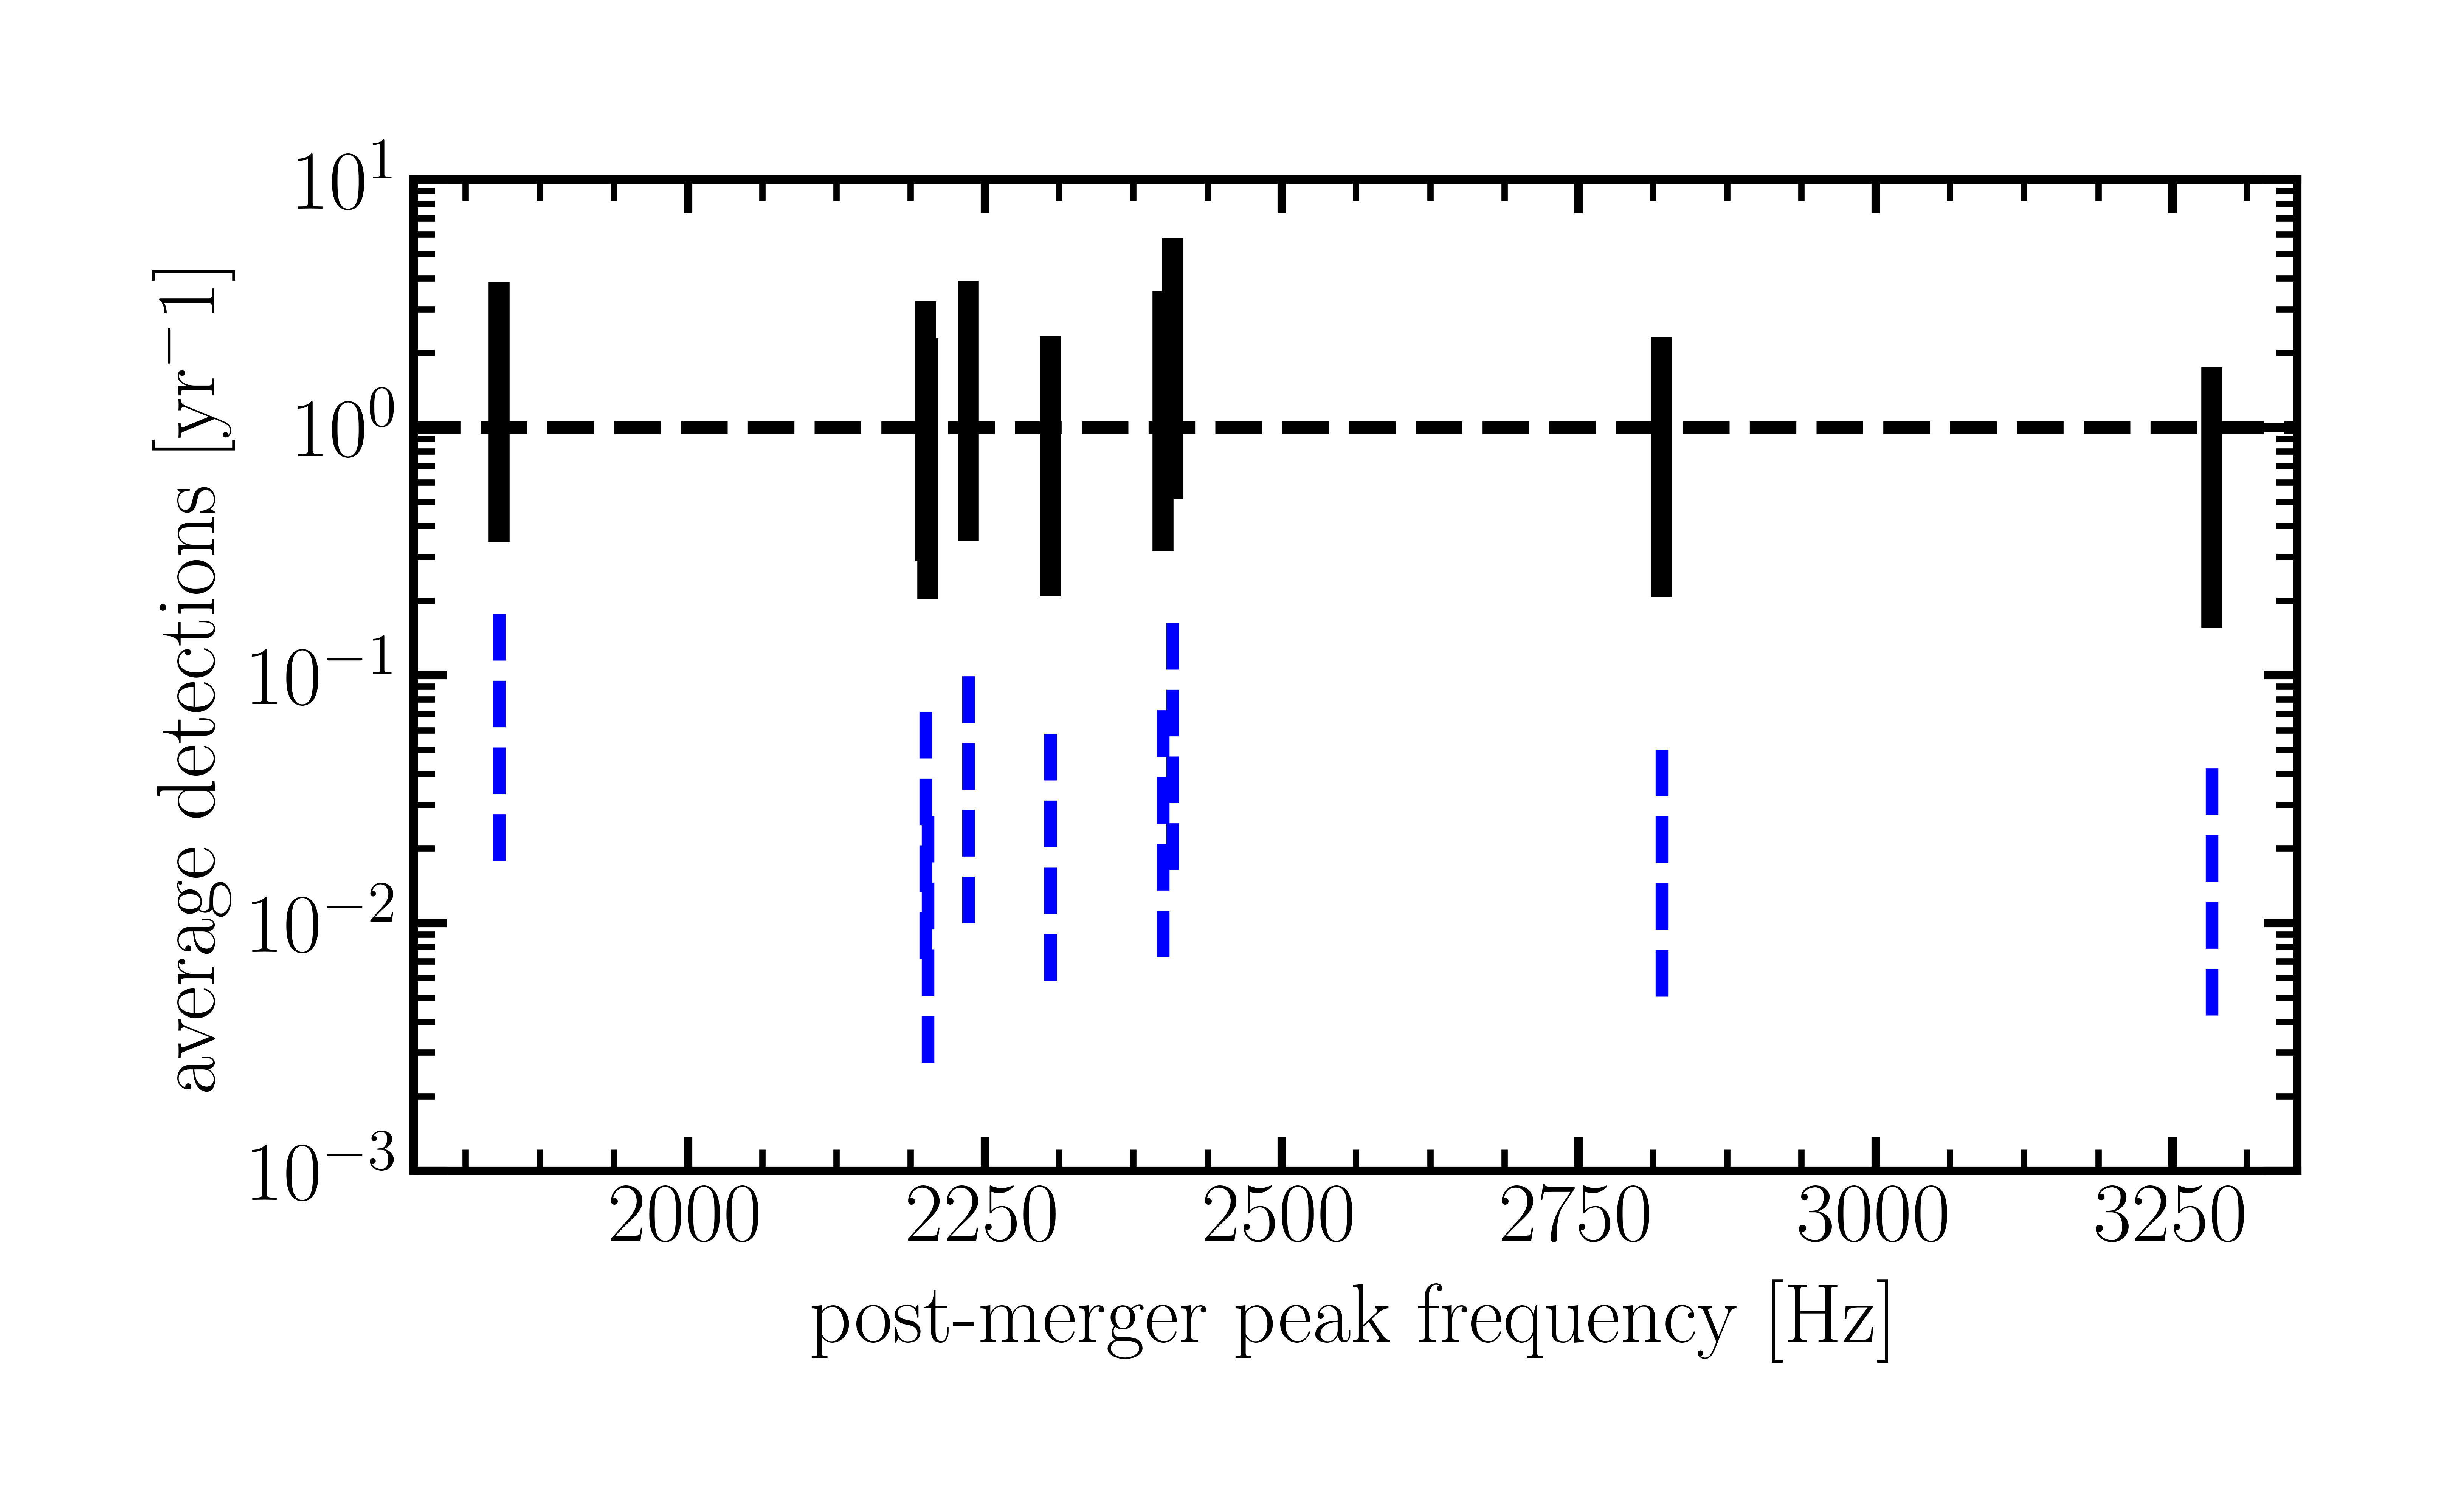
\includegraphics[width=0.5\textwidth]{post_merger_rate.png}
\caption{The expected number of post-mergers signals per year with matched-filter signal-to-noise ratio $\rho_\text{mf}>5$ as a function of peak gravitational-wave frequency.
In dashed blue, we show the number of detections for Network I with two A+ observatories while black indicates the number of detections for Network II when we add OzHF to make a three-detector network.
The length of the vertical lines shows the 90\% credible interval owing to uncertainty from the binary neutron star merger rate~\cite{GW190425}.}
\label{fig:ndet}
\end{figure}

Figure~\ref{fig:ndet} clearly shows that the average number of detections per year for a network of A+ interferometers \textit{not} including an EMO is significantly below one.  Put another way, one would have to wait potentially many tens of years for a first post-merger detection without an EMO.  That number increases to an average of about one detection per year with an EMO, ranging anywhere from one every few years to a few per year.  We emphasise that the uncertainty here encodes our uncertainty in the binary neutron star merger rate.


\subsection{Other Science}
Neutron-star science is the key science driver for an EMO.
Since the natural timescale for neutron-star physics is ${\cal O}(\unit[1]{ms})$, the frequency of gravitational waves from binary neutron star mergers is well-matched to an EMO.
Recent observations of binary neutron star mergers~\cite{abbott17_gw170817_detection, GW190425} make neutron-star science low-risk because there is no doubt that binary neutron stars merge frequently enough for EMO science.
The measurement of matter effects in binary neutron stars will facilitate additional science, for example, breaking degeneracies in measurements of the Hubble flow~\cite{messenger12} and helping to distinguish between neutron stars and black holes~\cite[e.g.,][]{fasano20}.

Additional sources {\em may} be within the reach of an EMO, for example, supernovae~\cite[e.g.,][]{powell19}, quasi-monochromatic signals from rotating neutron stars~\cite[e.g.,][]{lasky15,riles17}, or more speculatively, superradiance from axion clouds~\cite{yoshino14}.
However the detectability (and/or existence) of these sources is more speculative, and hence the great scientific impact of these targets must be tempered with theoretical uncertainty.
Other sources such as binary black holes and the stochastic background are more easily studied at lower frequencies; an EMO can detect them, but no better than broadband observatory such as A+.

By expanding the observing band of gravitational-wave networks, an EMO will explore a new region of parameter space.
History suggests that opening a new window on the Universe often yields unexpected discoveries; gamma-ray bursts are a great example~\cite{grb1977}.
While an EMO may detect something totally surprising, we can be confident that it will measure the properties of matter effects in neutron stars.

\section{Conclusion}\label{sec:conclusion}
We present the technology requirements and key science drivers for an Extreme Matter Observatory: a high-frequency gravitational-wave observatory optimized to study nuclear physics with merging neutron stars.  An EMO utilises high-circulating laser power and quantum squeezing to achieve necessary high-frequency noise, while sacrificing difficult and costly low-frequency sensitivity.  Reaching a strain sensitivity of $\approx\unit[10^{-24}]{1/\sqrt{Hz}}$ in the $\sim$1--$\unit[3]{kHz}$ regime allows gravitational waves from the post-merger remnant of a binary neutron star collision to be detected with sufficient regularity.  Such an EMO should operate simultaneously with the A+ network which drives the sky localisation of sources and enables rapid electromagnetic identification of neutron star merger counterparts.  The combination of electromagnetic observations, such as those achieved for GW170817, together with precision gravitational-wave observations of the inspiral, merger, \textrm{and} post-merger remnant will provide unprecedented insight into both the \textrm{hot} and cold equations of state of nuclear matter at supranuclear densities.

The want for a heterogeneous network of interferometers drives the timescale for an EMO. Realistically, such a detector could be operational in the late 2020s and early 2030s, giving sufficient time for co-operations with the A+ network while impacting technology development for third-generation detectors.  Such a proposal relies on engineering and detector design studies to be funded and implemented soon.

The location of an EMO is less critical than that of broadband detectors, where the network relies on long baselines to increase sky localization accuracy.  One suitable location includes Australia, where the OzHF concept~\cite{bailes19} sees the four-kilometer EMO eventually extended into a $\sim10$-km-scale, broadband Cosmic Explorer South; the need for which has been identified by the Gravitational Wave International Committee.

\bibliography{bibfile}

\end{document}



